\documentclass[10pt, a4paper]{article}

%% Language and font encodings
\usepackage[brazil]{babel}
\usepackage[utf8x]{inputenc}
\usepackage[T1]{fontenc}

%% Sets page size and margins
\usepackage[a4paper,top=3cm,bottom=2cm,left=3cm,right=3cm,marginparwidth=1.75cm]{geometry}

%% Useful packages
\usepackage{amsmath}
\usepackage{graphicx}
\usepackage[colorinlistoftodos]{todonotes}
\usepackage[colorlinks=true, allcolors=blue]{hyperref}


\title{IF678 - Infraestrutura de Comunicação}
\author{Íris Soares}

\begin{document}
\maketitle

\begin{figure} [h]
\centering
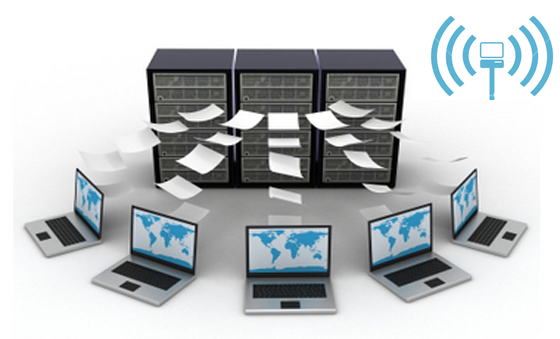
\includegraphics[height=9cm]{iss3.png}
\caption{By VVMSS2 [CC BY-SA 3.0], from Wikimedia Commons}
\end{figure}
% Link da imagem: 
% <https://commons.wikimedia.org/wiki/File:Redes_inf10.png>

\section{Introdução}

A disciplina de Infra-Estrutura de Comunicação está inserida na área de Redes, e é destinada ao ensino do que são e de como funcionam redes e protocolos de comunicação, e à aplicação desses conhecimentos na implementação de redes de computadores. Para tanto, a disciplina é dividida em cinco módulos que particionam todo o conteúdo: Introdução às redes de Computadores, que trata dos conceitos mais básicos e introdutórios como “o que é a internet? O que é um protocolo?” e temas como a história da internet no Brasil e no mundo; Camada de aplicação, que traz os princípios das aplicações de redes, trata de alguns protocolos de rede e construção de servidores web; Camada de Transporte, que aborda tipos diferentes de transferência de dados, serviços da camada de transporte e formas de fazer o controle de congestionamento; Camada de rede, que trata desde o que é um roteador à circuitos virtuais e o Protocolo de Internet; e por fim, o módulo de Camada de Enlace, que trata dos sistemas de detecção e correção de erros, Ethernet, Hubs e Stwiches.\cite{jk}

\section{Relevância}

A disciplina tem papel fundamental no curso para que o aluno compreenda os mais variados aspectos de projetos e implementação de redes de computadores, assim como o funcionamento da internet e dos diversos protocolos de comunicação existentes, ou seja, o aluno terá um bom entendimento da rede mundial de computadores e de como ela funciona.

\section{Relação com outras disciplinas}

Essa disciplina faz parte da tríade hardware, software e comunicação. Essas três cadeiras (Infra-Estrutura de Hardware, Infra-Estrutura de Software e Infra-Estrutura de Comunicação) são a base para a construção de qualquer sistema de computação atual, e, portanto possuem uma relação interdisciplinar entre si.\\[0.5cm]

\begin{table}[h]
\centering
\begin{tabular}{|l|p{8cm}|} \hline
\textbf{Cadeira} & \textbf{Relação Interdisciplinar}\\\hline
IF674 - Infraestrutura de Hardware & Enquanto Infra-Estrutura de Comunicação tem por objetivo fazer o aluno entender os diversos aspectos de projetos e implementação de redes de computadores, Infra-Estrutura de Hardware tem por objetivo dar uma visão geral dos componentes de um computador, e os princípios de funcionamentos de cada um dos componentes. Além dos conceitos mais básicos, também são lecionados conceitos avançados, técnicas usadas nos processadores comerciais atuais que garantem um grande aumento no desempenho da máquina. De forma global, o objetivo da disciplina é fazer com que o aluno passe a entender os diversos aspectos de projetos e implementação de computadores e que esse conhecimento possa ajudar em tarefas de sua vida profissional.\\\hline
IF677 - Infraestrutura de Software & Infra-Estrutura de Software, por sua vez tem a finalidade de apresentar os conceitos e sistemas de software básicos de um computador, promover o entendimento sobre o funcionamento dos sistemas de software que fornecem suporte para aplicativos (como jogos e navegadores Web) interagirem com o hardware, se relacionando, desse modo, tanto com Infra-Estrutura de Comunicação quanto com Infra-Estrutura de Hardware, integrando-os.\\\hline
\end{tabular}
\caption{Disciplinas que se relacionam à IfraEstrutura de Comunicação}
\end{table}

\bibliographystyle{alpha}
\bibliography{iss3}

\end{document}